% Diploma creator template. Reads results.csv. 
% Made for Instanssi demoparty.
% 2013 Tuomo Sipola (tuomo.sipola@iki.fi)

\documentclass[14pt,a4paper,onecolumn,oneside]{extarticle}

% UTF-8 source code.
\usepackage[T1]{fontenc}
\usepackage{xltxtra}

% Set language.
\usepackage{polyglossia}
\setdefaultlanguage{finnish}
%\setotherlanguages{italian,latin,greek,hebrew}

% Set font.
\defaultfontfeatures{Mapping=tex-text, Numbers=Lining, Scale=MatchLowercase, Ligatures=Common}
\setmainfont{Exo Bold}

% Colors.
\usepackage{xcolor}
\definecolor{instanssiblue}{RGB}{80,167,244}
\definecolor{instanssigrey}{RGB}{72,72,72}

\newcommand{\bluehilight}[1]{{\fontspec{Exo Black}{\textcolor{instanssiblue}{#1}}}}
\newcommand{\greyhilight}[1]{{\fontspec{Exo Black}{\textcolor{instanssigrey}{#1}}}}

% Page margins.
\usepackage[margin=4cm]{geometry}

% Background frame.
\usepackage[center]{background}
\SetBgAngle{0}
\SetBgScale{1}
\SetBgPosition{8cm,-12.3cm}
\SetBgContents{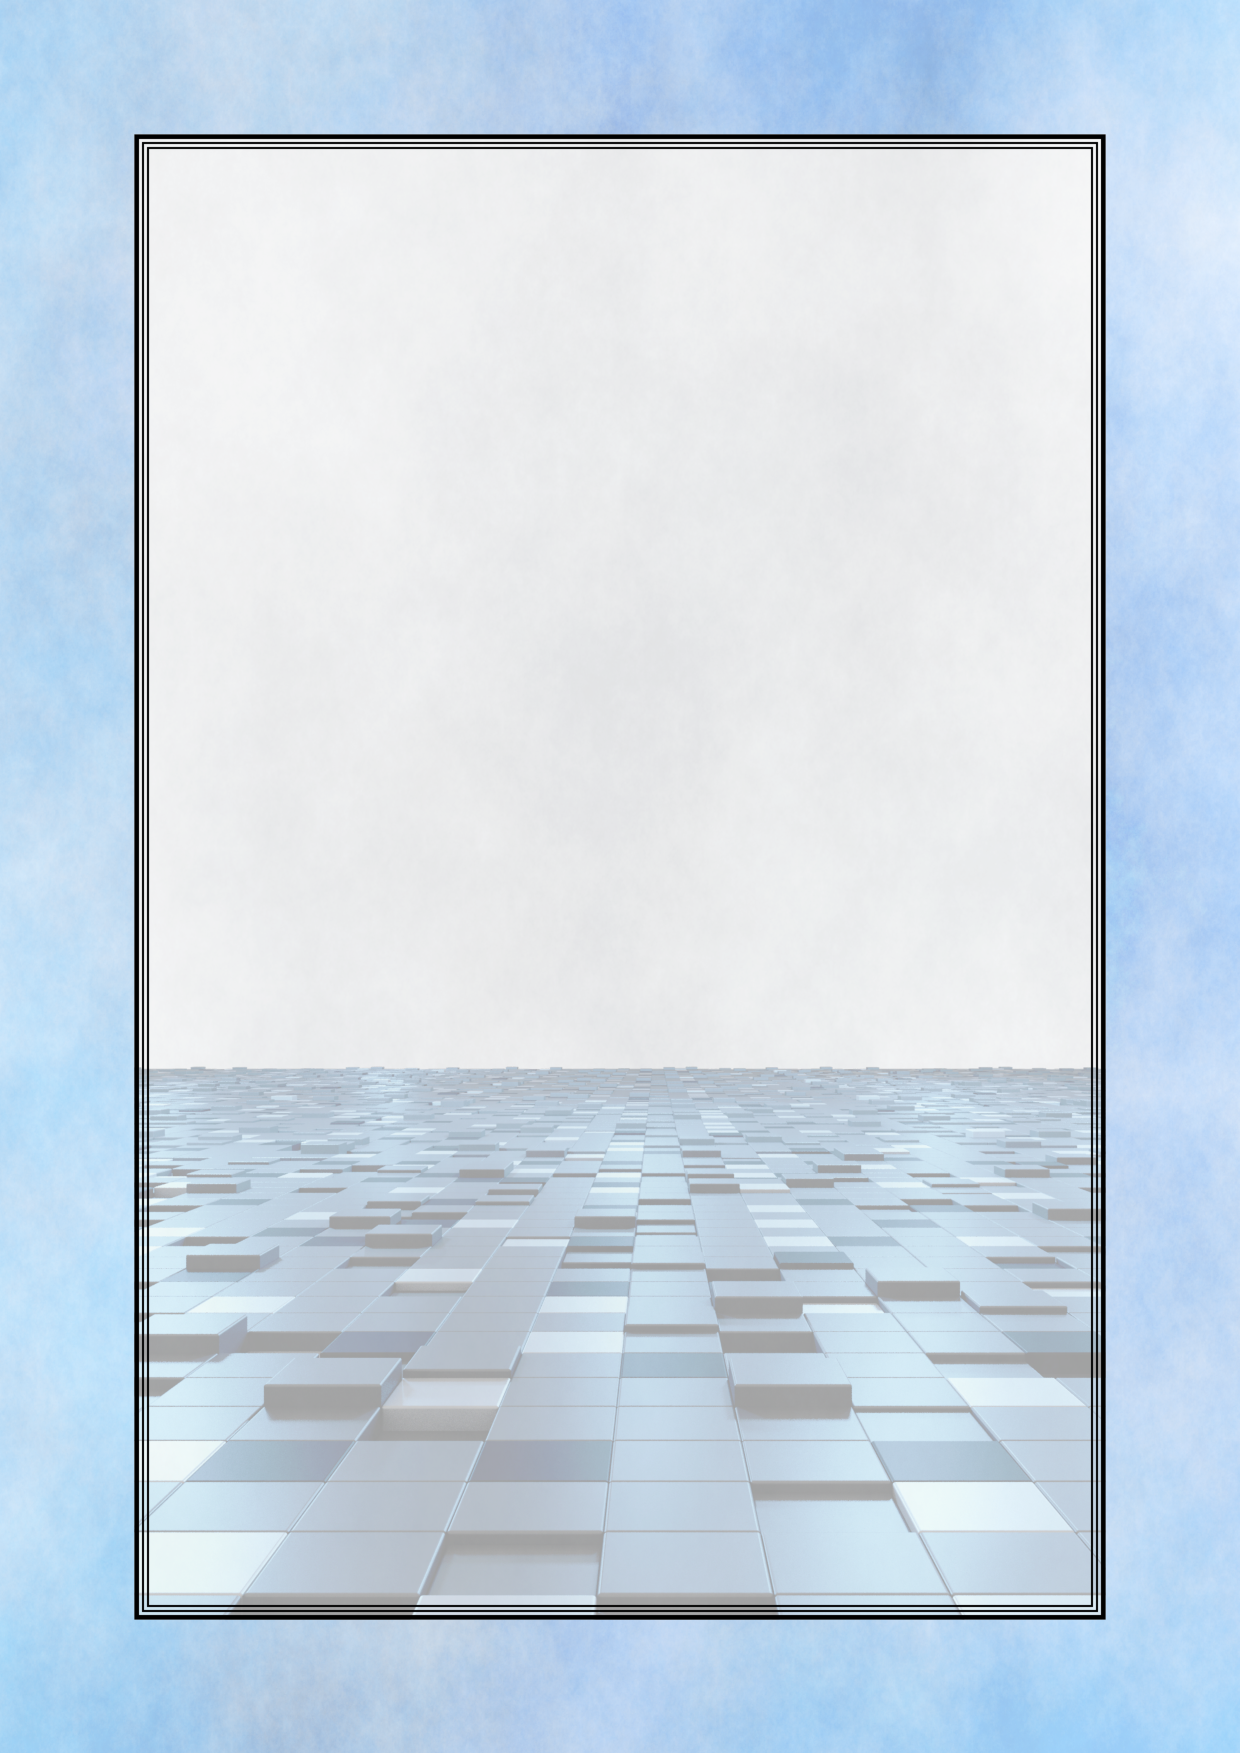
\includegraphics{frame.pdf}}

% To read CSV and do mail merging.
\usepackage{csvtools}

% Compare strings.
\usepackage{xstring}

%\usepackage[pdftex]{graphicx}

\begin{document}
\pagestyle{empty}
\applyCSVfile{results.csv}{%

\begin{center}

\mbox{}
\vspace{0.1\textheight}

\Huge\greyhilight{\insertAuthor} \\

\vspace{0.6em}

\IfStrEq{true}{\insertHasEntry}{%
\normalsize
\IfStrEq{true}{\insertHasMultipleAuthors}{OVAT}{ON}
\MakeUppercase{teoksella} \\

\vspace{0.4em}

\Huge
\bluehilight{\insertEntry} \\
}{}

\vspace{0.6em}

\normalsize
\IfStrEq{true}{\insertHasMultipleAuthors}{SIJOITTUNEET}{SIJOITTUNUT} \\

\vspace{1.5em}

\Huge
\insertPlacement \\

\vspace{1em}

\normalsize
\MakeUppercase{sijalle Instanssi 2013 -tapahtuman kilpasarjassa} \\

\vspace{1em}

\Large
\insertCompo \\

\vspace{1em}

\normalsize
\MakeUppercase{ja täten}
\IfStrEq{true}{\insertHasMultipleAuthors}{OSOITTANEET}{OSOITTANUT} 
\MakeUppercase{erinomaista pätevyyttä ja taitoa digitaalisen tekemisen saralla.} \\

\vspace{1em}

\vfill

\textcolor{instanssiblue}{Linkki Jyväskylä ry:n ja Instanssin puolesta} \\

\end{center}

\bigskip

\small
\noindent \rule{6cm}{1pt} \hfill \rule{6cm}{1pt} \\
\noindent Simo Haatainen \hfill Joel Lehtonen \\
\noindent \textcolor{instanssigrey}{(työryhmän puheenjohtaja)} \hfill \textcolor{instanssigrey}{(kompovastaava)} \\

\newpage

}
\end{document}

